\chapter[Deseño]{
  \label{chp:disenho}
  Deseño
}
\minitoc
\newpage

\section{Descrición do funcionamento}

O sistema consiste nunha páxina web con apartados adicados, por un lado, ao que chamamos actividades de consumo, e por outro ás actividades de produción.

\subsection{Actividades de consumo de contidos}

Son aquelas levadas a cabo polos ouvintes das emisoras e os programas presentes no sistema. Un usuario, no seu papel de \say{consumidor}, pode, mediante a interface web, acceder ao catálogo de programas, xa sexa mediante as ferramentas de busca proporcionadas ou mediante as recomendacións que a propia páxina amosa en portada.

Dentro da páxina correspondente a unha emisora, o usuario atopará un reprodutor HTML5 desde o que escoitar a súa emisión en directo mediante streaming. O usuario terá opción de facerse \say{seguidor} da emisora para acceder a ela de xeito máis rápido desde a páxina principal.

Tamén obterá acceso a lista de programas emitidos por dita emisora co seu horario de emisión. Na páxina de cada programa verá a lista completa de episodios dispoñibles e terá a opción de subscribirse para poder acceder de xeito máis rápido aos novos episodios publicados.

Na páxina propia de episodio atopará outro reprodutor HTML que lle posibilitará ou ben a escoita por streaming ou ben a descarga directa do ficheiro de audio correspondente. Poderá votar o programa a favor ou en contra (isto repercutirá na popularidade do programa, concepto explicado máis adiante) e deixar un comentario no caso de que esta opción esté habilitada polos administradores do programa.


\subsection{Actividades de produción de contidos}

Son aquelas levadas a cabo polos donos e administradores dos programas e emisoras. Un usuario, no seu papel de produtor, poderá engadir ao sistema unha nova emisora cubrindo o formulario habilitado a tal efecto na interface web no que deberá introducir manualmente os datos.

Poderá tamén engadir un programa. Para isto, o usuario só necesitará proporcionarlle ao sistema un enlace ao ficheiro de RSS do podcast que queira engadir e o sistema encargarase de extraer a información tanto dos programas coma dos episodios correspondentes. Este programa e os seus episodios manteranse actualizados xa que o propio backend do sistema comprobará periodicamente se houbo algún cambio no RSS e actualizará a base de datos de xeito acorde.  

Un usuario que posúa un programa ou emisora pode invitar a outro usuario a colaborar na xestión desta ou deste.

\section{Arquitectura}

A elección de Django coma framework de desenvolvemento obriga a seguir o patrón Modelo-Vista-Template. Este patrón é unha pequena variación do máis coñecido Modelo-Vista-Controlador, que define 3 capas interconectadas coa fin de separar a lóxica da aplicación(Vista) do almacenamento dos datos(Modelo) e estas dúas, á súa vez, da interface de usuario(Controlador). A vantaxe que ofrecen os \say{templates} de Django é a posibilidade de utilizar os tipos propios do framework para implementar certa lóxica presentacional no renderizado do template.

Neste proxecto, os modelos  definíronse no módulo models.py e as vistas en views.py. Trataranse coma paquetes nos seguintes diagramas. A capa template ven definida no paquete de templates.

\begin{figure}[h]
	\centering
	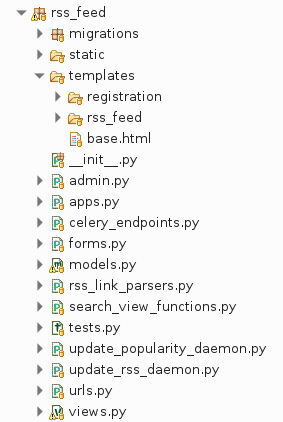
\includegraphics[scale=0.5,keepaspectratio=true]{./images/project_tree.png}
	\caption{Módulos do proxecto.}
	\label{fig:project_tree}
\end{figure}


\section{Capa Modelo}

Á hora de definir esta cuestión, tratáronse de respectar as regras do modelo relacional de bases de datos, porén, fixeronse algunhas excepcións motivadas por esixencia da elección do framework Django:

\begin{itemize}
	\item Claves primarias subrogadas: Django encárgase da identificación das tuplas engadindo ás táboas un campo numérico enteiro de incremento automático. Isto utilizarase en todas as táboas sen excepción.
	
	\item Relación 1-1: Como se ve no diagrama Entidade-Relación da figura \ref{fig:diagrama_er}, existe unha relación 1-1 entre a entidade User e a súa entidade feble UserProfile. O motivo da existencia desta última é que se decidiu utilizar a entidade de usuario nativa de Django, co cal fíxose necesaria unha nova táboa para cubrir os atributos de usuario necesarios especificamente para o proxecto. 
\end{itemize}

No diagrama Entidade-Relación da figura \ref{fig:diagrama_er} pódense ver as táboas empregadas sen incluir aquelas automáticamente xeradas para o correcto funcionamento de Django e Celery a excepción da xa mencionada User. Por motivos de claridade, non se incluíron os atributos agás aqueles adicionais nas táboas correspondentes ás relacións \say{N a N}.

A estrutura da BD tradúcese na aplicación ás clases definidas no paquete models.py que se ve na figura \ref{fig:clase_models}. Por claridade, nese diagrama de clases só se incluíron os atributos máis representativos ou explicativos das relacións entre clases.

\begin{figure}[h]
	\centering
	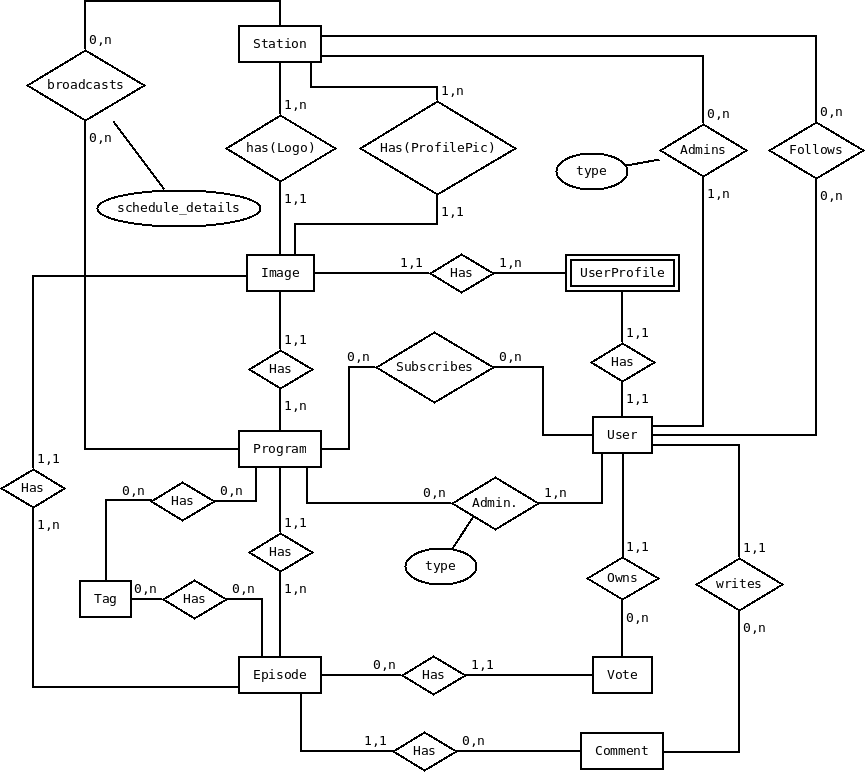
\includegraphics[scale=0.5,keepaspectratio=true]{./images/ER_diagrama.png}
	\caption{Diagrama Entidade-Relación da Base de Datos.}
	\label{fig:diagrama_er}
\end{figure}

\begin{figure}[h]
	\centering
	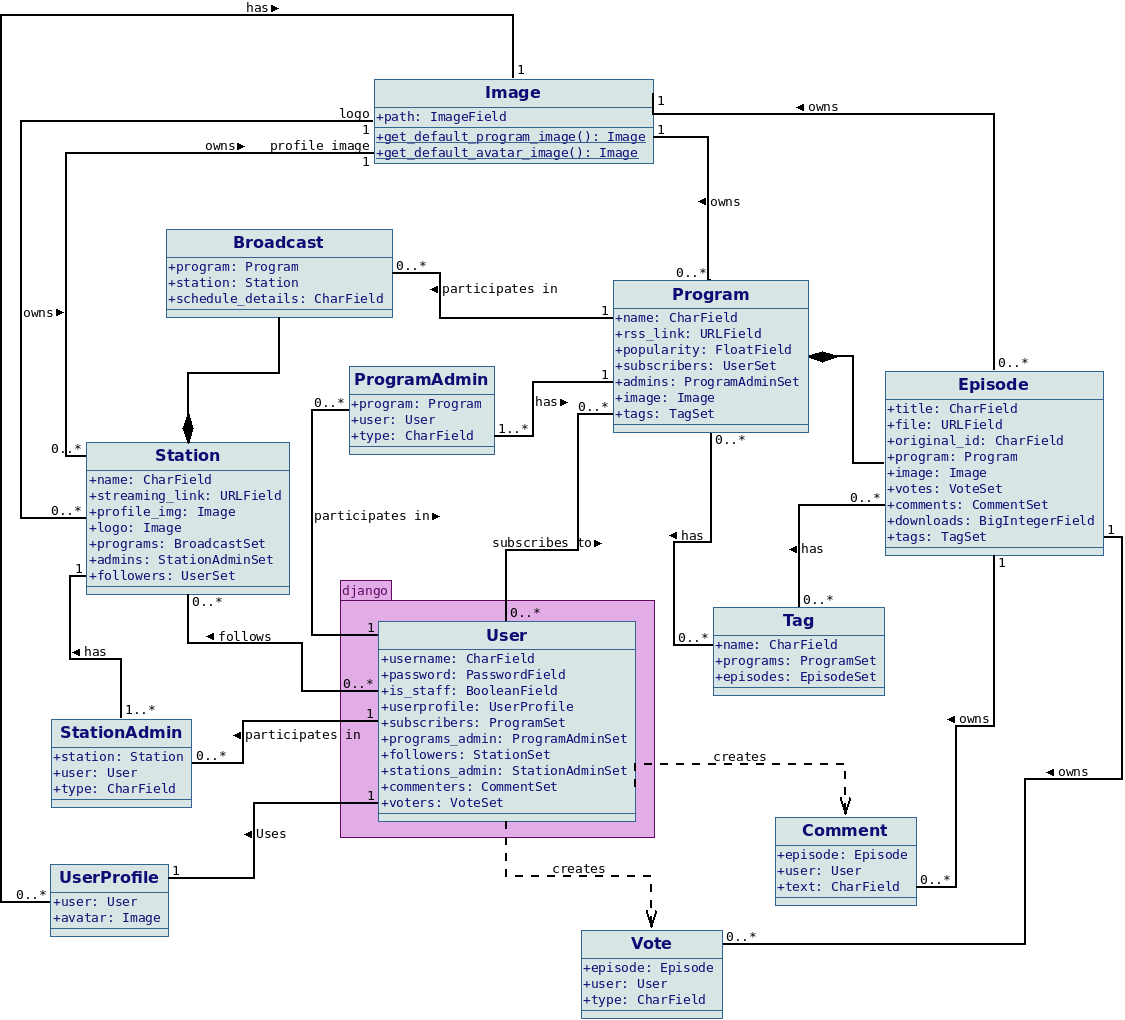
\includegraphics[scale=0.4,keepaspectratio=true]{./images/class_diagram.png}
	\caption{Diagrama de clases do paquete models.}
	\label{fig:clase_models}
\end{figure}


\begin{figure}[h]
	\centering
	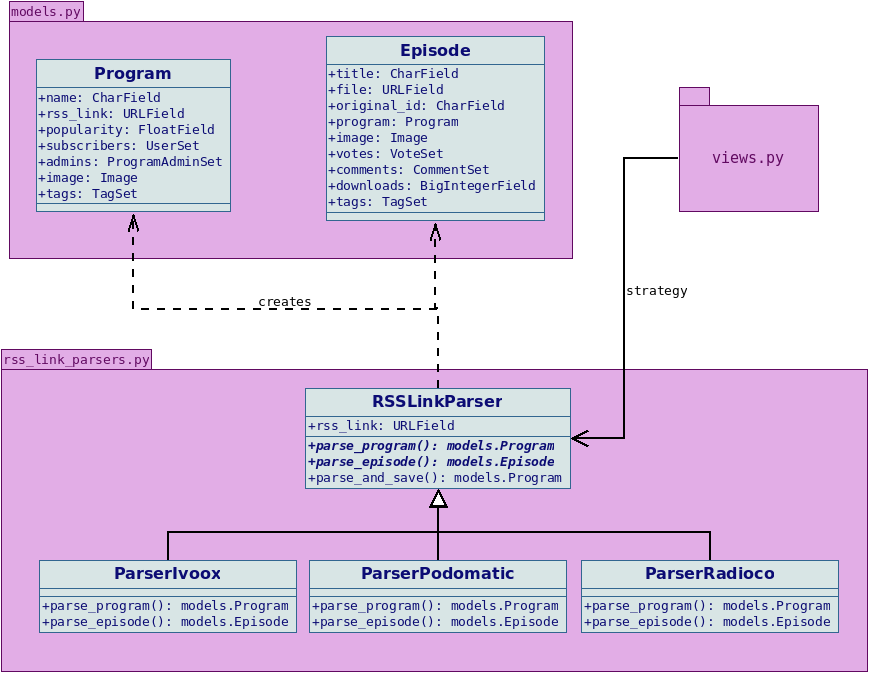
\includegraphics[scale=0.5,keepaspectratio=true]{./images/strategy.png}
	\caption{Patrón Estratexia utilizado para o procesamento de RSS.}
	\label{fig:strategy}
\end{figure}


\subsection{Os usuarios}

Os usuarios están definidos por dúas táboas: User e UserProfile que se corresponden coas clases User, do paquete django.contrib.auth.models, e UserProfile, definida polo desenvolvedor e, polo tanto, includida no paquete models.py. Esta segunda considerámola coma feble de User pois a existencia dun perfil está vencellada de xeito ineludible á existencia dun usuario.




